\documentclass[tikz]{standalone}

\usepackage{amsmath}
\usepackage{physics}

\usetikzlibrary{arrows.meta,backgrounds,fit,positioning}

\begin{document}
	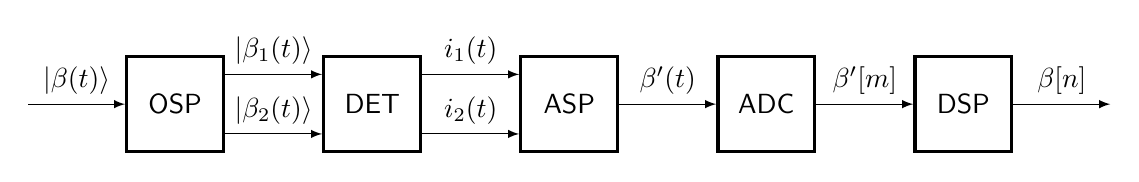
\begin{tikzpicture}[
		node distance=3.5em,
		arrow/.style={-latex},
		block/.style={draw, very thick, fill=white, minimum height=8ex, minimum width=3.5em},
	]
		\coordinate (in) at (0,0);
		\node (osp) [block, right=of in] {\textsf{OSP}};
		\node (det) [block, right=of osp] {\textsf{DET}};
		\node (asp) [block, right=of det] {\textsf{ASP}};
		\node (adc) [block, right=of asp] {\textsf{ADC}};
		\node (dsp) [block, right=of adc] {\textsf{DSP}};
		\coordinate[right=of dsp] (out);
		
		\draw[arrow] (in) -- (osp) node[midway, above]{$\ket{\beta(t)}$};
		\draw[arrow] ([yshift=2.5ex]osp.east) -- ([yshift=2.5ex]det.west) node[midway, above]{$\ket{\beta_1(t)}$};
		\draw[arrow] ([yshift=-2.5ex]osp.east) -- ([yshift=-2.5ex]det.west) node[midway, above]{$\ket{\beta_2(t)}$};
		\draw[arrow] ([yshift=2.5ex]det.east) -- ([yshift=2.5ex]asp.west) node[midway, above]{$i_1(t)$};
		\draw[arrow] ([yshift=-2.5ex]det.east) -- ([yshift=-2.5ex]asp.west) node[midway, above]{$i_2(t)$};
		\draw[arrow] (asp) -- (adc) node[midway, above]{$\beta^\prime(t)$};
		\draw[arrow] (adc) -- (dsp) node[midway, above]{$\beta^\prime[m]$};
		\draw[arrow] (dsp) -- (out) node[midway, above]{$\beta[n]$};
	\end{tikzpicture}
\end{document}
